\documentclass[12pt]{article}
% \title{Assignment 1: CS 754, Advanced Image Processing}
\author{\textbf{Question 3}}
\date{}
\usepackage{amsmath}
\usepackage{amssymb}
\usepackage{hyperref}
\usepackage{ulem}
\usepackage{enumitem}
\usepackage{float}
\usepackage{graphicx}
\usepackage{subcaption}
\usepackage{bm}
\usepackage{enumitem}
\pagenumbering{gobble}

\usepackage[margin=0.5in]{geometry}
\begin{document}
\maketitle

\begin{itemize}
    \item In this task, you will you use the well-known package L1\_LS from \url{https://stanford.edu/~boyd/l1_ls/}. This package is often used for compressed sensing solution, but here you will use it for the purpose of tomographic reconstruction. The homework folder contains images of two slices taken from an MR volume of the brain. Create measurements by parallel beam tomographic projections at any 18 randomly angles chosen from a uniform distribution on $[0,\pi)$. Use the MATLAB function `radon' for this purpose. Now perform tomographic reconstruction using the following method: (a) filtered back-projection using the Ram-Lak filter, as implemented in the `iradon' function in MATLAB, (b) independent CS-based reconstruction for each slice by solving an optimization problem of the form $J(\boldsymbol{x}) = \|\boldsymbol{y}-\boldsymbol{Ax}\|^2 + \lambda \|\boldsymbol{x}\|_1$, (c) a coupled CS-based reconstruction that takes into account the similarity of the two slices using the model given in the lectures notes on tomography. For parts (b) and (c), use the aforementioned package from Stanford. For part (c), make sure you use a \emph{different} random set of 18 angles for each of the two slices. The tricky part is careful creation of the forward model matrix $\boldsymbol{A}$ or a function handle representing that matrix, as well as the corresponding adjoint operator $\boldsymbol{A}^T$. Use the 2D-DCT basis for the image representation. Modify the objective function from the lecture notes for the case of three similar slices. Carefully define all terms in the equation but do not re-implement it. 
 \textsf{[3+7+8+7 = 25 points]}
\end{itemize}
\vspace*{0.5cm}\\
\textbf{Answer:} \\

\textbf{Using 18 different angles of projection }
\begin{enumerate}[label = (\alph*)]
    \item In this part we perform the reconstruction using the filtered back-projection method using Ram-Lak filter. The results are shown in the figure below. \\
    \textbf{Note:} For this part we have used 18 uniformly spaced angles of projection.
    \begin{figure}[H]
        \centering
        \begin{minipage}{.45\textwidth}
            \centering
            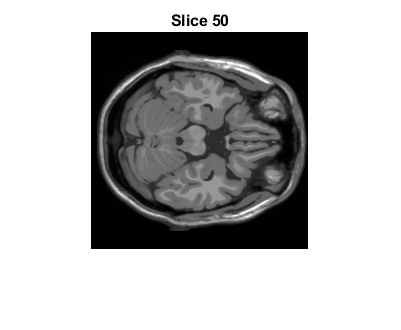
\includegraphics[width=\linewidth]{Images/Q3_50.png}
            \caption*{Original Slice 50}
        \end{minipage}
        \begin{minipage}{.45\textwidth}
            \centering
            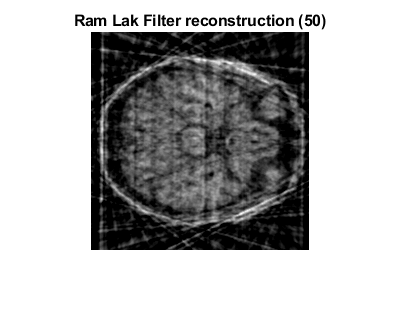
\includegraphics[width=\linewidth]{Images/Q3_50_a.png}
            \caption*{Reconstructed Slice 50 using Ram-Lak filter}
        \end{minipage}
    \end{figure}
    \begin{figure}[H]
        \centering
        \begin{minipage}{.45\textwidth}
            \centering
            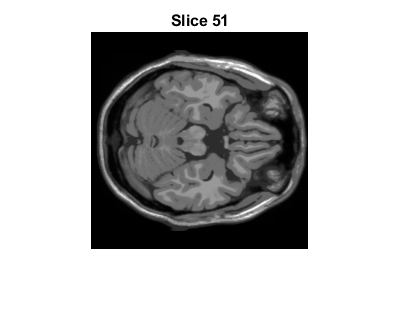
\includegraphics[width=\linewidth]{Images/Q3_51.png}
            \caption*{Original Slice 51}
        \end{minipage}
        \begin{minipage}{.45\textwidth}
            \centering
            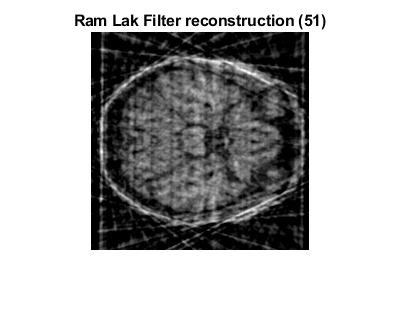
\includegraphics[width=\linewidth]{Images/Q3_51_a.png}
            \caption*{Reconstructed Slice 51 using Ram-Lak filter}
        \end{minipage}
    \end{figure}

    \item In this part we have performed independent Compressed Sensing reconstruction for each slice. The optimization problem solved here is
    \begin{gather*}
        J(x) = || y-Ax ||^2_2 + \lambda ||x||_1
    \end{gather*}
    The results are shown in the figure below. \\
    \textbf{Note:} For this part we have used 18 uniformly spaced angles of projection.
    \begin{figure}[H]
        \centering
        \begin{minipage}{.45\textwidth}
            \centering
            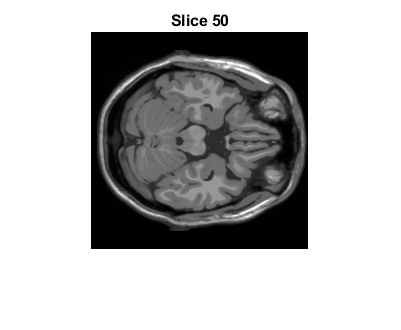
\includegraphics[width=\linewidth]{Images/Q3_50.png}
            \caption*{Original Slice 50}
        \end{minipage}
        \begin{minipage}{.45\textwidth}
            \centering
            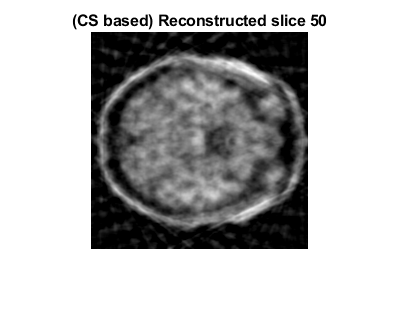
\includegraphics[width=\linewidth]{Images/Q3_50_b.png}
            \caption*{CS based reconstruction (Slice 50) }
        \end{minipage}
    \end{figure}
    \begin{figure}[H]
        \centering
        \begin{minipage}{.45\textwidth}
            \centering
            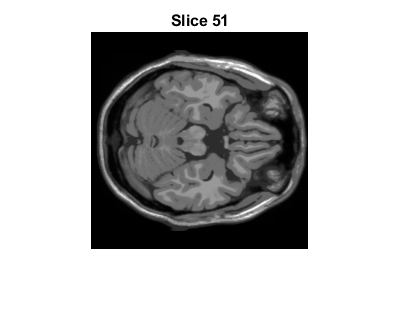
\includegraphics[width=\linewidth]{Images/Q3_51.png}
            \caption*{Original Slice 51}
        \end{minipage}
        \begin{minipage}{.45\textwidth}
            \centering
            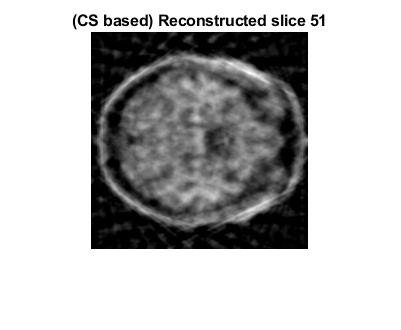
\includegraphics[width=\linewidth]{Images/Q3_51_b.png}
            \caption*{CS based reconstruction (Slice 51)}
        \end{minipage}
    \end{figure}

    \item In this part we perform a coupled CS-based reconstruction. The optimization problem solved here is
    \begin{gather*}
        E(\beta_1 , \beta_2) =  \left \lVert \begin{pmatrix} y_1 \\ y_2 \end{pmatrix} - \begin{pmatrix} R_1U & 0 \\ R_2U & R_2U \end{pmatrix}  \begin{pmatrix} \beta_1 \\ \Delta \beta \end{pmatrix}\right\rVert^2_2 + \lambda  \left \lVert\begin{pmatrix} \beta_1 \\ \Delta \beta \end{pmatrix} \right\rVert_1 
    \end{gather*}
    where, \\
    \begin{itemize}
        \item $ \begin{pmatrix} y_1 \\ y_2 \\ \end{pmatrix} $ is the measurement vector, \\
        \item $ \begin{pmatrix} R_1U & 0 \\ R_2U & R_2U \end{pmatrix} $ is the forward model matrix where U represents the inverse 2D DCT matrix and $R_1$ and $R_2$ are the radon projection matrices,\\
        \item $ \begin{pmatrix} \beta_1 \\ \Delta \beta \end{pmatrix} $ is the vector of unknown parameters \\
    $ \Delta \beta = \beta_2 - \beta_1 $ is the difference between the two unknown parameters.
\end{itemize}
    The result of the reconstruction is shown in the figure below. \\
    \textbf{Note:} For this part we have used 18 randomly generated angles of projection.
    \begin{figure}[H]
        \centering
        \begin{minipage}{.45\textwidth}
            \centering
            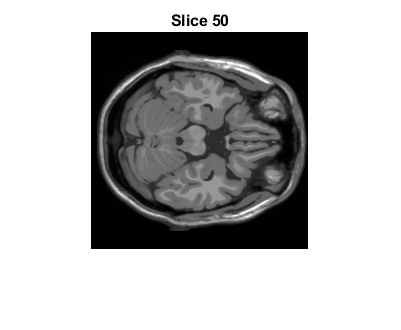
\includegraphics[width=\linewidth]{Images/Q3_50.png}
            \caption*{Original Slice 50}
        \end{minipage}
        \begin{minipage}{.45\textwidth}
            \centering
            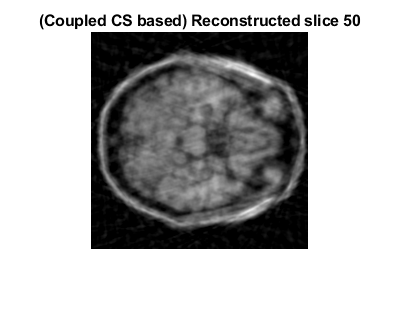
\includegraphics[width=\linewidth]{Images/Q3_50_c.png}
            \caption*{Coupled CS based reconstruction (Slice 50) }
        \end{minipage}
    \end{figure}
    \begin{figure}[H]
        \centering
        \begin{minipage}{.45\textwidth}
            \centering
            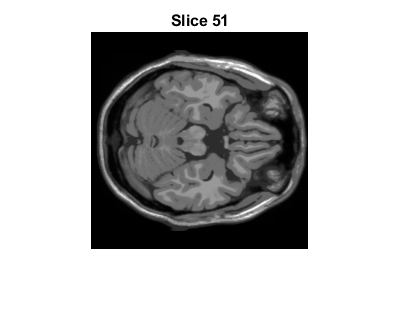
\includegraphics[width=\linewidth]{Images/Q3_51.png}
            \caption*{Original Slice 51}
        \end{minipage}
        \begin{minipage}{.45\textwidth}
            \centering
            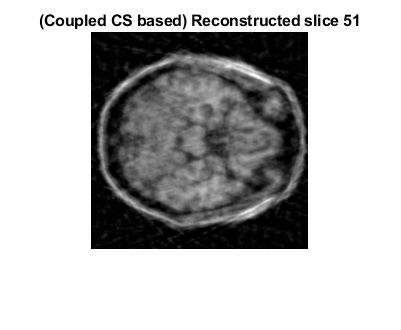
\includegraphics[width=\linewidth]{Images/Q3_51_c.png}
            \caption*{Coupled CS based reconstruction (Slice 51)}
        \end{minipage}
    \end{figure}

    \item In this part we derive the optimization problem for the coupled CS-based reconstruction using 3 consecutive slices. The optimization problem we solve is given as 
    \begin{gather*}
        E(\beta_1, \beta_2, \beta_3) = \left \lVert y_1 - R_1U \beta_1 \right\rVert^2_2 + \left \lVert y_2 - R_2U \beta_2\right\rVert^2_2 + \left \lVert y_3 - R_3U \beta_3\right\rVert^2_2 + \lambda \left \lVert \beta_1\right\rVert_1 + \lambda \left \lVert \beta_2 - \beta_1\right\rVert_1 + \lambda \left \lVert \beta_3 - \beta_1\right\rVert_1  \\
        = \left \lVert \begin{pmatrix} y_1 \\ y_2 \\ y_3 \end{pmatrix} - \begin{pmatrix} R_1U & 0 & 0 \\ R_2U & R_2U & 0 \\ R_3U & 0 & R_3U \end{pmatrix} \begin{pmatrix} \beta_1 \\ \Delta \beta_1 \\ \Delta \beta_2 \end{pmatrix}\right\rVert^2_2 + \lambda \left \lVert\begin{pmatrix} \beta_1 \\ \Delta \beta_1 \\ \Delta \beta_2 \end{pmatrix} \right\rVert_1
    \end{gather*}
    where, \\
    \begin{itemize}
        \item $ \begin{pmatrix} y_1 \\ y_2 \\ y_3 \\ \end{pmatrix} $ is the measurement vector, \\
        \item $ \begin{pmatrix} R_1U & 0 & 0 \\ R_2U & R_2U & 0 \\ R_3U & 0 & R_3U \end{pmatrix} $ is the forward model matrix where U represents the inverse 2D DCT matrix and $R_1$ and $R_2$ and $R_3$ are the radon projection matrices,\\
        \item $ \begin{pmatrix} \beta_1 \\ \Delta \beta_1 \\ \Delta \beta_2 \end{pmatrix} $ is the vector of unknown parameters \\
    $ \Delta \beta_1 = \beta_2 - \beta_1 $ and $ \Delta \beta_2 = \beta_3 - \beta_1 $ are the difference between the two unknown parameters.
    \end{itemize}
\end{enumerate}

\textbf{EXTRA PART}

To check the results that we get by using more angles of projection, we used 30 angles of projection. Let us see the results.\\ 
\textbf{Using 30 different angles of projection}
\begin{enumerate}[label = (\alph*)]
    \item FBP with Ram-Lak filter
    \begin{figure}[H]
        \centering
        \begin{minipage}{.45\textwidth}
            \centering
            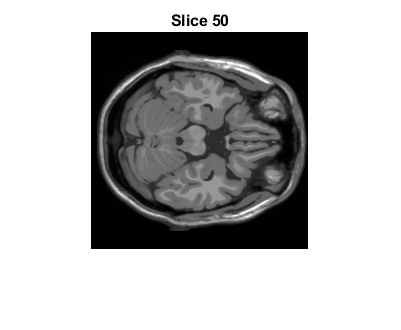
\includegraphics[width=\linewidth]{Images/Q3_50.png}
            \caption*{Original Slice 50}
        \end{minipage}
        \begin{minipage}{.45\textwidth}
            \centering
            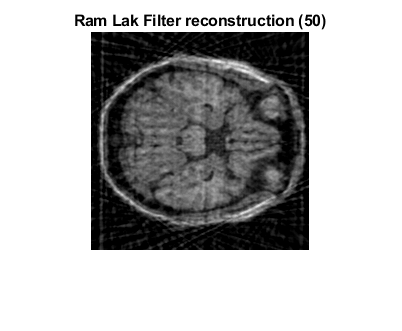
\includegraphics[width=\linewidth]{Images/Q3_Extra_50_a.png}
            \caption*{Reconstructed Slice 50 using Ram-Lak filter}
        \end{minipage}
    \end{figure}
    \begin{figure}[H]
        \centering
        \begin{minipage}{.45\textwidth}
            \centering
            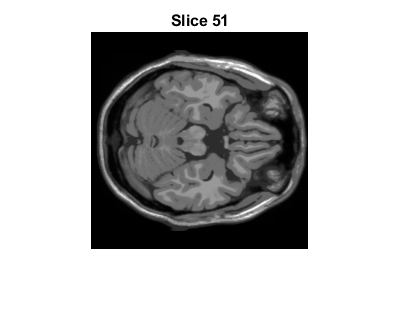
\includegraphics[width=\linewidth]{Images/Q3_51.png}
            \caption*{Original Slice 51}
        \end{minipage}
        \begin{minipage}{.45\textwidth}
            \centering
            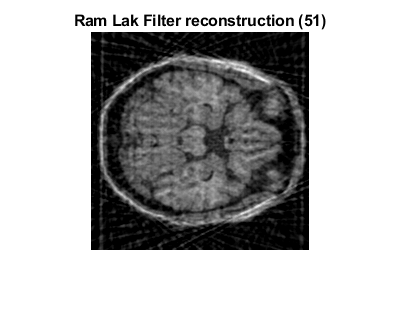
\includegraphics[width=\linewidth]{Images/Q3_Extra_51_a.png}
            \caption*{Reconstructed Slice 51 using Ram-Lak filter}
        \end{minipage}
    \end{figure}    

    \item CS based independent reconstruction
    \begin{figure}[H]
        \centering
        \begin{minipage}{.45\textwidth}
            \centering
            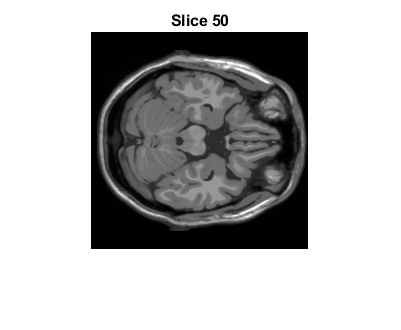
\includegraphics[width=\linewidth]{Images/Q3_50.png}
            \caption*{Original Slice 50}
        \end{minipage}
        \begin{minipage}{.45\textwidth}
            \centering
            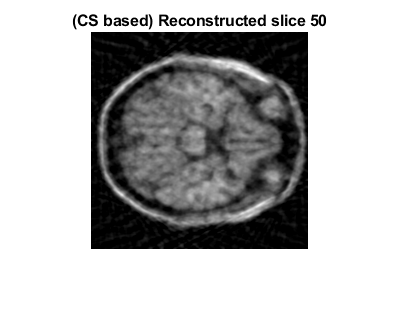
\includegraphics[width=\linewidth]{Images/Q3_Extra_50_b.png}
            \caption*{CS based independent reconstruction}
        \end{minipage}
    \end{figure}
    \begin{figure}[H]
        \centering
        \begin{minipage}{.45\textwidth}
            \centering
            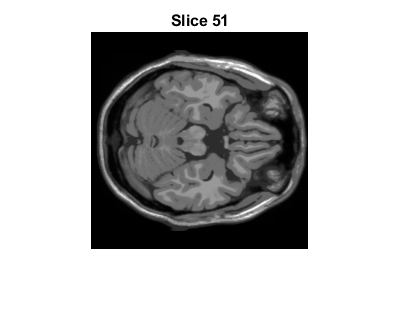
\includegraphics[width=\linewidth]{Images/Q3_51.png}
            \caption*{Original Slice 51}
        \end{minipage}
        \begin{minipage}{.45\textwidth}
            \centering
            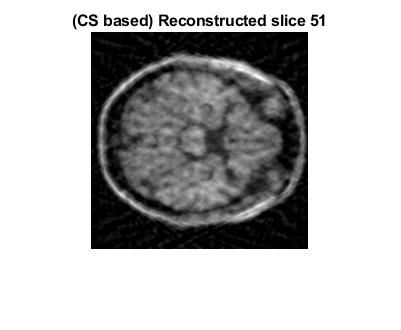
\includegraphics[width=\linewidth]{Images/Q3_Extra_51_b.png}
            \caption*{CS based independent reconstruction}
        \end{minipage}
    \end{figure}

    \item CS based coupled reconstruction
    \begin{figure}[H]
        \centering
        \begin{minipage}{.45\textwidth}
            \centering
            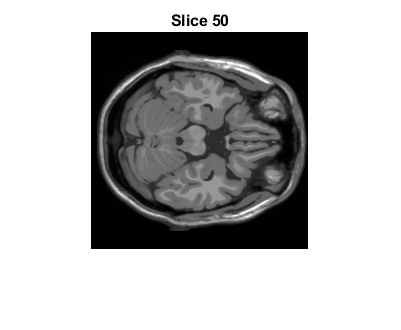
\includegraphics[width=\linewidth]{Images/Q3_50.png}
            \caption*{Original Slice 50}
        \end{minipage}
        \begin{minipage}{.45\textwidth}
            \centering
            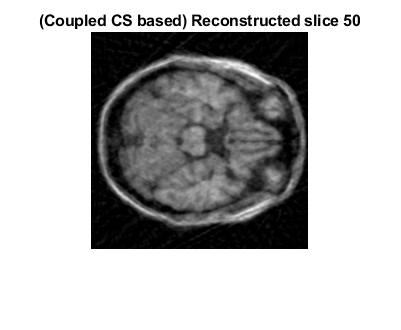
\includegraphics[width=\linewidth]{Images/Q3_Extra_50_c.png}
            \caption*{CS based coupled reconstruction}
        \end{minipage}
    \end{figure}
    \begin{figure}[H]
        \centering
        \begin{minipage}{.45\textwidth}
            \centering
            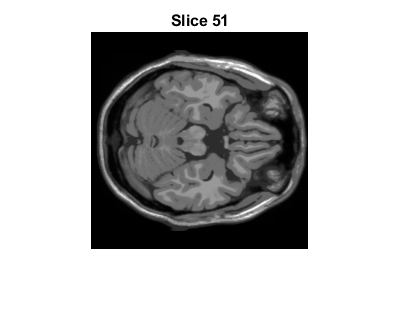
\includegraphics[width=\linewidth]{Images/Q3_51.png}
            \caption*{Original Slice 51}
        \end{minipage}
        \begin{minipage}{.45\textwidth}
            \centering
            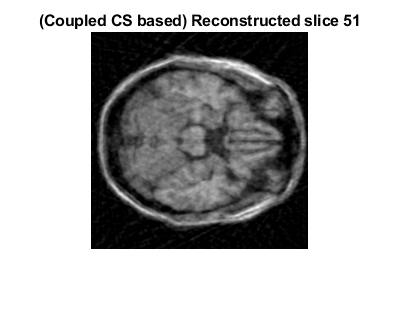
\includegraphics[width=\linewidth]{Images/Q3_Extra_51_c.png}
            \caption*{CS based coupled reconstruction}
        \end{minipage}
    \end{figure}
    \end{enumerate}
    
    Here we can easily that the reconstruction using the coupled scheme is better than the independent scheme. Also, as the number of projection angles is increased the reconstruction quality is also improved.
\end{document}
